% Transition vers une application TEI Publisher pour les éditions en ligne EHRI

\section{Analyse des besoins}

\subsection{Profil des utilisateur$\cdot$ice$\cdot$s}
L'objectif principal de l'EHRI est de soutenir la recherche sur la Shoah, notamment en éditant des corpus thématiques. Les collections rassemblent des documents d'archives conservés dans les institutions partenaires du projet. De ce fait, les éditions de l'EHRI s'adressent plutôt à un public de chercheur$\cdot$euse$\cdot$s et d'étudiant$\cdot$e$\cdot$s, particulièrement en Histoire.


\subsection{Transposer les fonctionnalités d'Omeka}
Le cahier des charges des éditions EHRI publiées avec Omeka a été rigoureusement étudié\footcite{Ehri2018}. La transition vers TEI Publisher ne peut se faire sans s'assurer que les fonctionnalités dont dispose Omeka sont également disponibles dans TEI Publisher. Nous avons donc identifié quels étaient les principaux critères recherchés par l'équipe éditoriale, puis nous avons parcouru la liste des \textit{web components} de TEI Publisher pour établir une correspondance~:

\begin{itemize}
    \item La possibilité d'ajouter une documentation à propos de l'édition (module \texttt{pb-mark -down})~;
    \item Une barre de recherche (module \texttt{pb-search})~;
    \item Une recherche facettée (modules \texttt{pb-browse-docs} et \texttt{pb-custom-form})~;
    \item Une transcription lisible et sans distraction (modules \texttt{pb-view}, \texttt{pb-collapse}, \texttt{pb-grid} et \texttt{pb-grid-action}~;
    \item La possibilité de télécharger les fichiers dans plusieurs formats, principalement XML, PDF et ePub (module \texttt{pb-download})~;
    \item La génération de cartes interactives (modules \texttt{pb-leaflet}, \texttt{pb-geolocation}, \texttt{pb-map-icon} et \texttt{pb-map-layer})~;
    \item L'affichage d'informations contextuelles au survol de la transcription (modules \texttt{pb-highlight} et \texttt{pb-popover}).
\end{itemize}



\section{Création du prototype d'application}

\subsection{Des fonctionnalités supplémentaires}
Notre exploration des modules mis à disposition par TEI Publisher nous a permis d'établir une liste de fonctionnalités supplémentaires que l'application TEI Publisher dédiée à EHRI pourrait présenter~: 

\begin{itemize}
    \item Une application disponible en plusieurs langues (module \texttt{pb-lang})~;
    \item Une chronologie des documents (module \texttt{pb-timeline})~;
    \item Une navigation claire à l'intérieur de la collection (module \texttt{pb-paginate}), ce que toutes les éditions EHRI avec Omeka ne proposent pas~;
    \item Une navigation claire et simple à l'intérieur du document, notamment entre le fac-similé et la transcription (module \texttt{pb-navigation})~;
    \item La possibilité de zoomer aisément sur le fac-similé sans perte de qualité (module \texttt{pb-facsimile})~;
\end{itemize}

Certaines de ces fonctionnalités sont déjà disponibles sur l'application DiScholEd et pourront donc être facilement implémentées.


\subsection{Maquettes visuelles}
À partir des fonctionnalités décrites, nous avons proposé des maquettes visuelles pour le futur développement de l'application~: 

\begin{figure}[h]
    \centering
    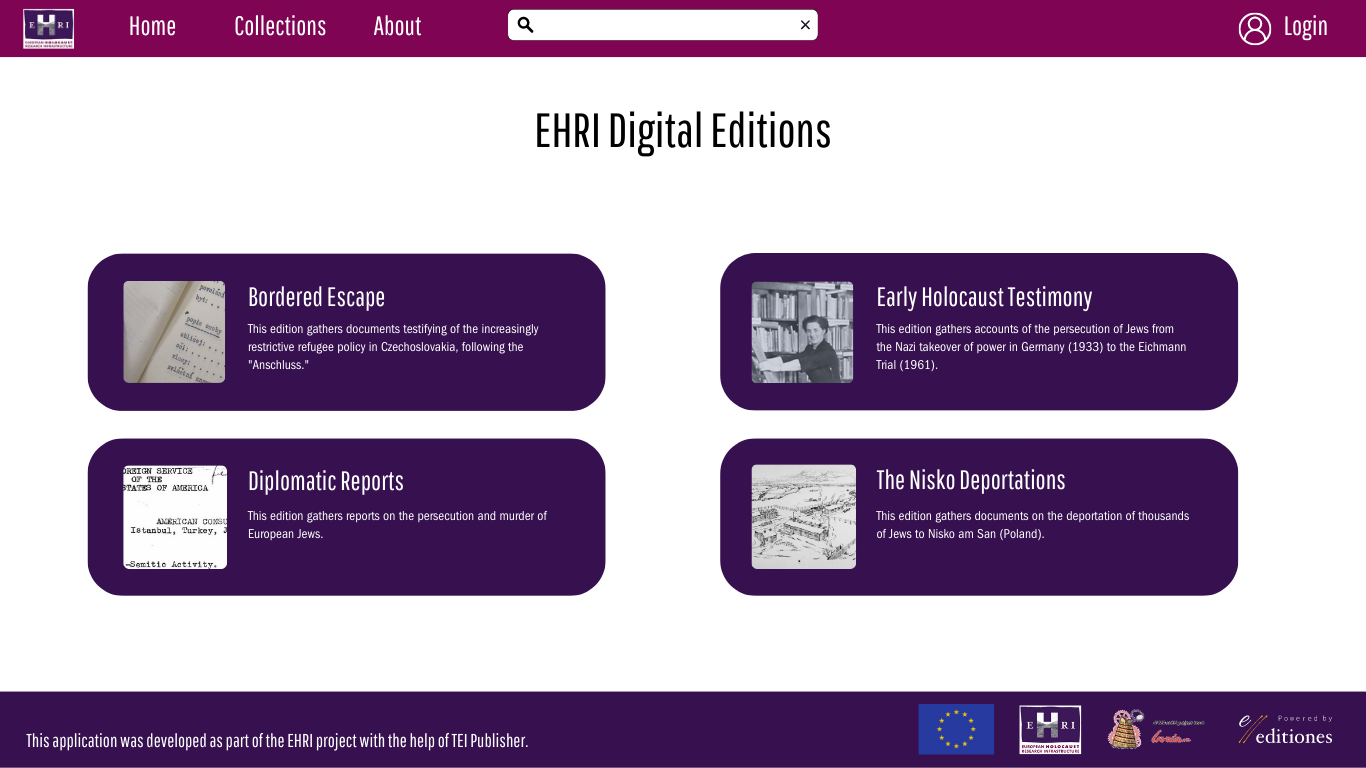
\includegraphics[width=0.55\linewidth]{2-MAIN/images/ehri-accueil.png}
    \caption{Maquette de la page d'accueil EHRI avec TEI Publisher}
    \label{fig:ehri-accueilmaquette}
\end{figure}

\begin{figure}[h]
    \centering
    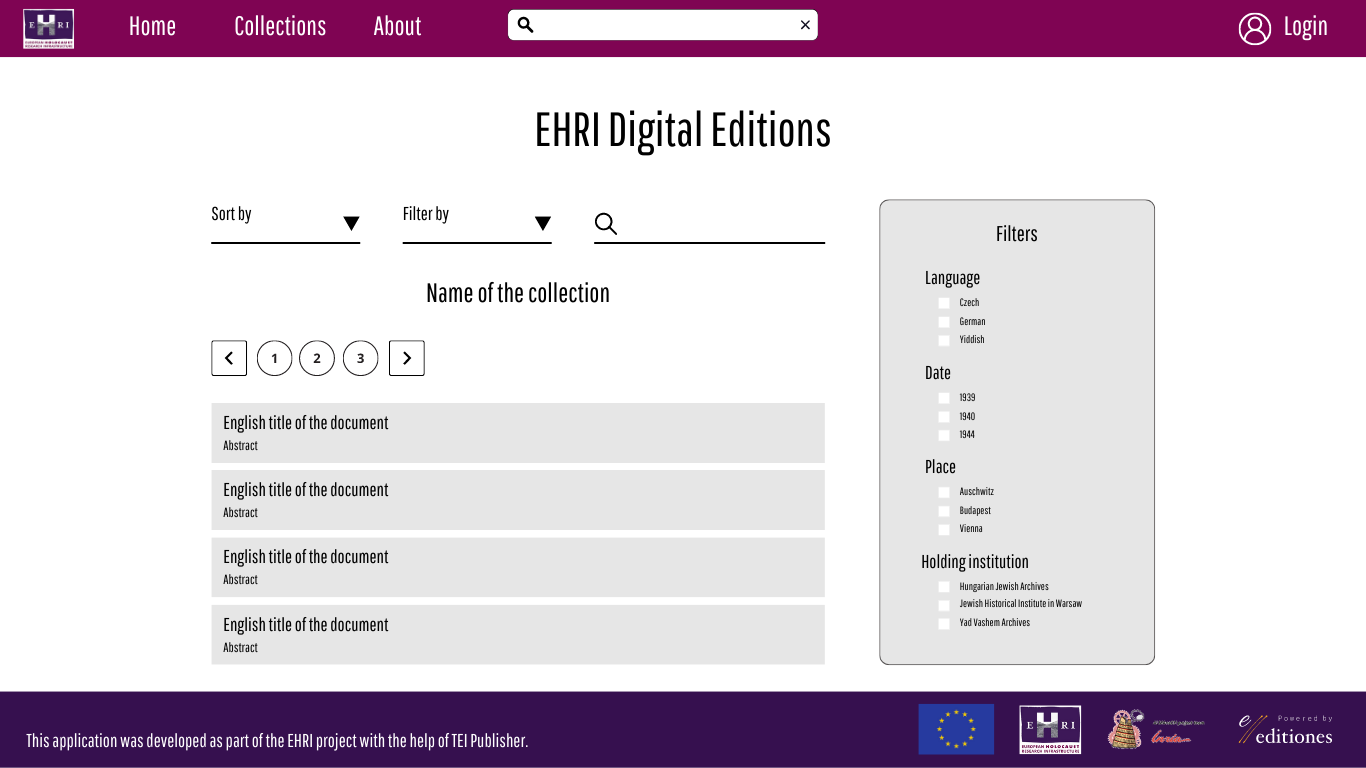
\includegraphics[width=0.55\linewidth]{2-MAIN/images/ehri-collection.png}
    \caption{Maquette de navigation dans la collection}
    \label{fig:ehri-collmaquette}
\end{figure}

\begin{figure}[h]
    \centering
    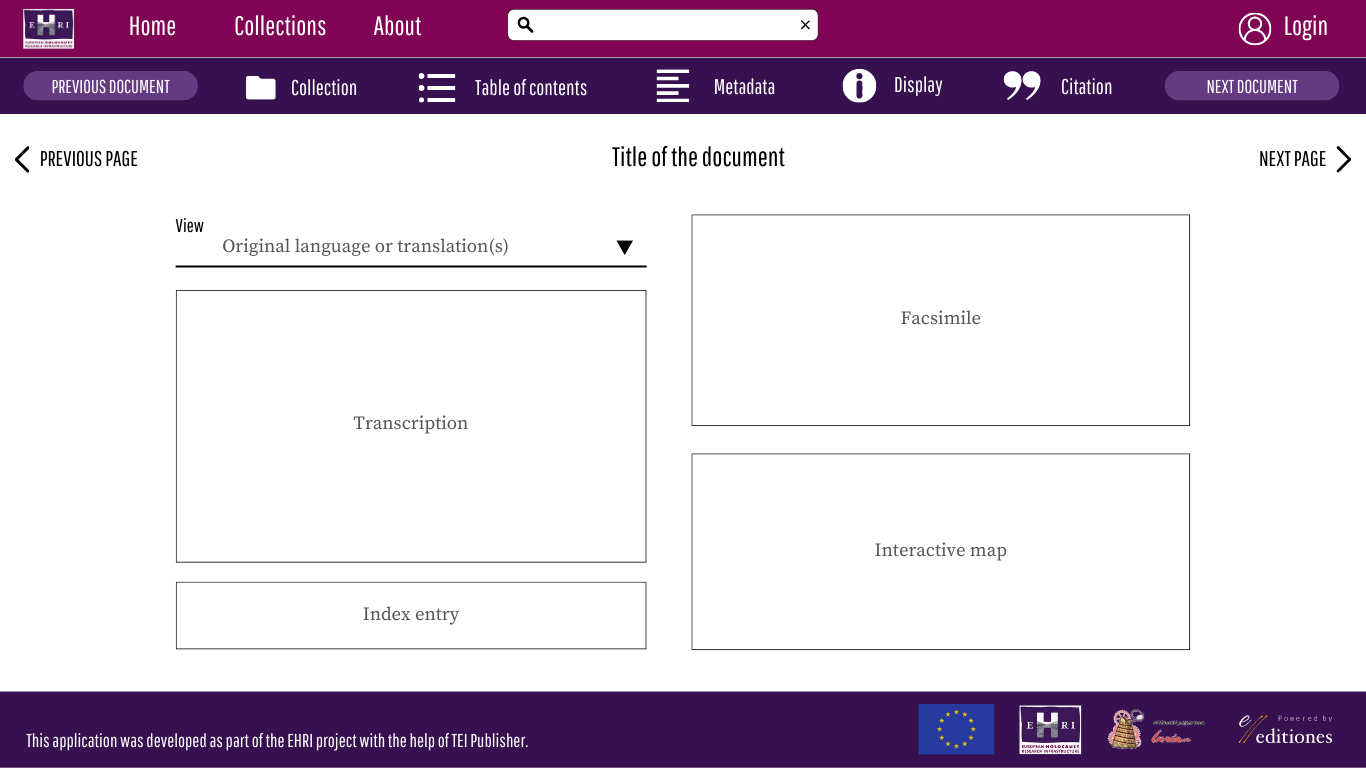
\includegraphics[width=0.55\linewidth]{2-MAIN/images/ehri-document.png}
    \caption{Maquette de l'affichage du document avec TEI Publisher}
    \label{fig:ehri-docmaquette}
\end{figure}

Notre équipe a commencé le développement de l'application TEI Publisher EHRI, dont le prototype devrait être présenté aux éditeur$\cdot$ice$\cdot$s du WP12 entre octobre et novembre prochains.

\begin{figure}[!h]
    \centering
    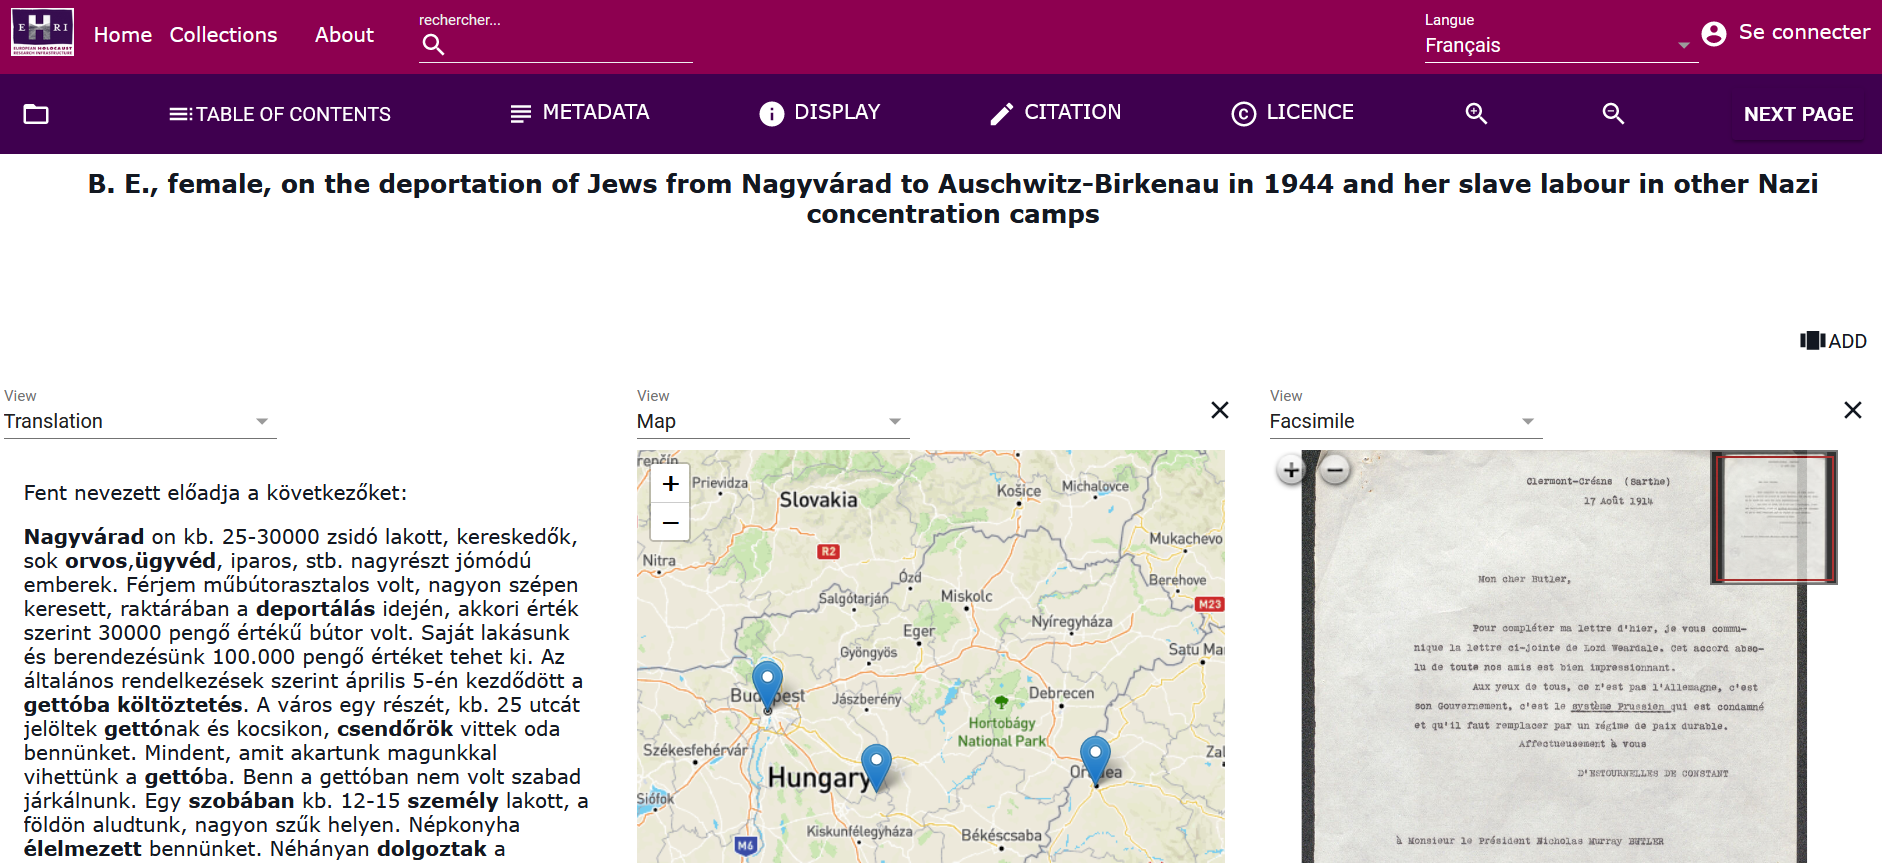
\includegraphics[width=1\linewidth]{2-MAIN/images/ehri-proofofconcept.png}
    \caption{Exemple de l'affichage d'un document sur l'application TEI Publisher EHRI}
    \label{fig:ehri-proofofconcept}
\end{figure}

Grâce à son affichage horizontal, TEI Publisher permet de profiter de trois vues simultanément sans perdre en confort de lecture (Figure \ref{fig:ehri-proofofconcept}). Les différentes vues sont par ailleurs modulables, c'est-à-dire que l'utilisateur$\cdot$ice peut choisir le nombre de vues souhaité et ce qu'elles affichent.